% !TeX program = pdflatex
% Báo cáo KT1 Ames Housing. Biên dịch pdfLaTeX hai lần.
\documentclass[12pt,a4paper]{article}
\usepackage{iftex}
\ifPDFTeX
\usepackage[T5]{fontenc}
\usepackage[utf8]{inputenc}
\usepackage{lmodern}
\else
\usepackage{fontspec}
\setmainfont{lmroman10-regular.otf}[BoldFont=lmroman10-bold.otf,ItalicFont=lmroman10-italic.otf,BoldItalicFont=lmroman10-bolditalic.otf]
\fi
\usepackage[vietnamese]{babel}
\usepackage[margin=2cm,headheight=15pt]{geometry}
\usepackage{amsmath,amssymb,bm}
\usepackage{graphicx,booktabs,tabularx,array,float,caption}
\usepackage{setspace,microtype,xurl}
\usepackage[unicode,hidelinks,pdftitle={Báo cáo KT1 Dự đoán giá nhà Ames},pdfauthor={Sinh viên bổ sung thông tin}]{hyperref}
\graphicspath{{images/}}
\setstretch{1.09}
\setlength{\parindent}{0pt}
\setlength{\parskip}{6pt}
\setlength{\emergencystretch}{2em}
\renewcommand{\arraystretch}{1.17}
\captionsetup{font=small,labelfont=bf,skip=5pt}
\newcolumntype{Y}{>{\raggedright\arraybackslash}X}
\newcommand{\R}{\mathbb{R}}
\hypersetup{pageanchor=false}
\begin{document}
\begin{titlepage}
\centering
{\LARGE\bfseries BÁO CÁO BÀI KIỂM TRA 1\par}
\vspace{0.6cm}
{\Large\bfseries Dự đoán giá bất động sản\\dựa trên đặc điểm nhà ở\par}
\vspace{0.5cm}
{\large Học phần Học máy\par}
{\large Học kỳ 1 năm học 2026--2027\par}
\vspace{0.9cm}
\begin{tabular}{ll}
Sinh viên: & \makebox[9cm]{\dotfill}\\[0.3cm]
Mã sinh viên: & \dotfill\\[0.3cm]
Lớp: & \dotfill\\[0.3cm]
Giảng viên: & \dotfill
\end{tabular}
\vspace{0.7cm}
\par Ngày 26 tháng 10 năm 2026
\vspace{0.7cm}
\begin{flushleft}
\textbf{Tóm tắt}


Báo cáo xác định bài toán hồi quy giá bán nhà và xây dựng quy trình khảo sát, làm sạch, mã hóa và chuẩn hóa dữ liệu Ames Housing. Bộ dữ liệu gồm 2.930 giao dịch, 82 cột. Sau khi loại định danh và thông tin chỉ chắc chắn khi chốt giao dịch, dự án sử dụng 77 đầu vào. Tập huấn luyện gồm 2.589 nhà bán trong năm 2006–2009; 341 nhà năm 2010 được giữ làm tập kiểm tra.


Kết quả KT1 là bộ dữ liệu sẵn sàng gồm 350 cột sau tiền xử lý, không còn giá trị thiếu trong ma trận. Các ngưỡng clipping, giá trị điền khuyết, tham số chuẩn hóa và danh mục mã hóa chỉ được học trên tập huấn luyện. Dữ liệu cho thấy giá lệch phải, chất lượng và diện tích ở có quan hệ mạnh với giá; đa cộng tuyến giữa một số biến garage tạo cơ sở nghiên cứu chính quy hóa.


Phạm vi mốc này gồm xác định bài toán, EDA và tiền xử lý. Chưa huấn luyện hoặc công bố kết quả so sánh Linear Regression, Ridge, Lasso và Elastic Net. Các mức RMSE nêu trong báo cáo là mục tiêu dự kiến cho giai đoạn sau.


\end{flushleft}\end{titlepage}
\hypersetup{pageanchor=true}\tableofcontents\clearpage

\section{Phát biểu bài toán và mục tiêu}

\subsection{Bối cảnh và đơn vị mẫu}

Bài toán là học có giám sát dạng hồi quy: từ đặc điểm một căn nhà, dự đoán giá giao dịch SalePrice theo USD. Một mẫu tương ứng một bản ghi giao dịch của nhà ở tại Ames, Iowa. Mô hình được định hướng sử dụng trước khi hoàn tất giao dịch, với giả định các đặc điểm vật lý đã được ghi nhận và tháng/năm định bán đã biết.


Đầu vào gồm diện tích đất và nhà, loại nhà, khu vực, chất lượng, tình trạng, năm xây dựng, thông tin tầng hầm, garage và tiện ích. Không đưa Order, PID hoặc SalePrice vào X. Bỏ thêm Sale Type và Sale Condition để giảm nguy cơ dùng thông tin hình thành khi chốt giao dịch. Các đánh giá chất lượng cũng cần được kiểm tra về thời điểm thu thập khi áp dụng thực tế.


Đầu ra gốc là $y=\mathrm{SalePrice}>0$. Giá trị dùng để tối ưu mô hình
dự kiến là $z=\ln(1+y)$; khôi phục giá bằng $y=\exp(z)-1$.
Dữ liệu không phải giá rao bán Việt Nam và không đại diện cho thị trường hiện nay.

\subsection{Mục tiêu và tiêu chí thành công}

\begingroup\small\setlength{\tabcolsep}{5pt}
\begin{tabularx}{\linewidth}{@{}YYY@{}}\toprule

\textbf{Mục tiêu} & \textbf{Chỉ số hoặc minh chứng} & \textbf{Mức dự kiến}\\

\midrule

Chuẩn bị dữ liệu tin cậy ở KT1 & Ma trận hữu hạn, không thiếu; không lẫn ID/nhãn & Đạt kiểm tra tự động\\

Dự đoán tốt trên thang log ở KT2 & RMSE log qua CV theo năm & \ensuremath{\leq} 0,18 và giảm \ensuremath{\geq} 10\% so với baseline\\

Giải thích sai số bằng tiền & MAE và RMSE theo USD & Báo cáo cùng baseline, chưa đặt ngưỡng tùy tiện\\

Theo dõi mức giải thích biến thiên & R\textsuperscript{2} trên giá gốc & Chỉ số bổ trợ, có thể âm\\

\bottomrule\end{tabularx}\endgroup\par


\begin{align}
\mathrm{RMSE}_{\log}&=\sqrt{\frac{1}{m}\sum_{i=1}^{m}
 \left[\ln(1+y_i)-\ln(1+\widehat y_i)\right]^2},\\
\mathrm{MAE}_{\mathrm{USD}}&=\frac{1}{m}\sum_{i=1}^{m}|y_i-\widehat y_i|.
\end{align}
Với dự đoán không âm, RMSE log tương đương RMSLE. Chỉ số nhấn mạnh sai số
tương đối trong phạm vi giá rộng; không thể chuyển trực tiếp 0,18 thành một
tỷ lệ lỗi cố định cho mọi căn nhà. MAE có đơn vị USD, dễ diễn giải.
RMSE USD nhạy hơn với sai số lớn. $R^2$ so với phương án dự đoán trung bình
trên tập đang đánh giá.


Mức 0,18 là mục tiêu đề xuất, không phải kết quả đã đạt. Baseline dự kiến là hằng số học từ trung bình log giá trên từng tập train; khi so sánh theo MAE có thể bổ sung hằng số trung vị giá. Giữ cùng fold và chỉ số cho mọi mô hình.


\clearpage

\section{Nguồn dữ liệu và từ điển}

\subsection{Nguồn gốc và điều kiện sử dụng}

Sử dụng tệp \path{AmesHousing.txt} do Dean De Cock công bố cùng bài báo năm 2011 trên Journal of Statistics Education [1]. Dữ liệu được tổng hợp từ Ames City Assessor's Office, mô tả nhà bán tại Ames trong giai đoạn 2006–2010. Tệp gốc được tải ngày 26/10/2026 từ trang JSE [2], giữ nguyên bytes ở data/raw/AmesHousing.tsv. Tài liệu định nghĩa biến nằm ở \path{DataDocumentation.txt} [3].


Tệp có 2.930 dòng, 82 cột: một nhãn, hai định danh và 79 biến khác. Dự án dùng 77 biến dự báo sau khi bỏ thêm hai biến giao dịch. Sau quy tắc chuẩn hóa schema có 34 biến số và 43 biến phân loại; sau pipeline có 350 cột, bao gồm cờ thiếu và one-hot.


Nguồn cung cấp dữ liệu cho giảng dạy nhưng chưa nêu giấy phép dữ liệu riêng rõ ràng trong các tệp đã đọc. Dự án ghi nguồn, không tự gán CC0/MIT hoặc suy diễn giấy phép của một gói R sang dữ liệu gốc. Bản sao được lưu cho bài tập học phần trong repo private. Chi tiết nguồn và checksum SHA-256 nằm ở \path{data/SOURCES.md} và \path{reports/summary.json}.


\subsection{Các biến quan trọng}

\begingroup\small\setlength{\tabcolsep}{5pt}
\begin{tabularx}{\linewidth}{@{}YYY@{}}\toprule

\textbf{Biến} & \textbf{Ý nghĩa và đơn vị} & \textbf{Vai trò}\\

\midrule

SalePrice & Giá giao dịch USD & Nhãn, log1p\\

PID và Order & Mã thửa đất và số thứ tự & Loại khỏi X\\

MS SubClass & Mã loại nhà, có thể có số 0 đầu & Phân loại\\

Neighborhood & Khu vực trong Ames & One-hot\\

Lot Frontage và Lot Area & Mặt tiền ft và diện tích đất ft\textsuperscript{2} & Biến số\\

Gr Liv Area & Diện tích ở trên mặt đất ft\textsuperscript{2} & Biến số\\

Overall Qual và Overall Cond & Chất lượng và tình trạng tổng thể 1–10 & Điểm thứ bậc dạng số\\

Year Built và Year Remod/Add & Năm xây và năm cải tạo & Biến số\\

Total Bsmt SF & Tổng diện tích tầng hầm ft\textsuperscript{2} & Biến số\\

Garage Cars và Garage Area & Sức chứa xe và diện tích garage ft\textsuperscript{2} & Biến số\\

Mo Sold và Yr Sold & Tháng và năm bán & Tháng phân loại, năm dạng số\\

Sale Type và Sale Condition & Loại và điều kiện giao dịch & Loại khỏi X\\

\bottomrule\end{tabularx}\endgroup\par

Từ điển đầy đủ 82 cột ở \path{docs/data_dictionary.csv} ghi tên, kiểu dữ liệu đọc từ TSV, thang đo theo nguồn, ý nghĩa, số mã NA, vai trò và hướng xử lý. Các mã chi tiết như Ex/Gd/TA hoặc RL/RM được lưu trong tài liệu nguồn, không suy đoán chỉ từ tên cột. Diện tích giữ đơn vị gốc; 1 ft\textsuperscript{2} xấp xỉ 0,092903 m\textsuperscript{2}.


\clearpage

\section{Khảo sát thống kê và phân bố}

Tất cả thống kê thăm dò và quan hệ giá trong phần này sử dụng tập train 2006–2009. Tập test năm 2010 không dùng để quyết định đặc trưng hoặc cấu hình. Các bảng mô tả số và phân loại đầy đủ được xuất vào \path{reports/tables/numeric_summary_train.csv} và \path{categorical_summary_train.csv}.


Trên train, giá nhỏ nhất là 13,100 USD, lớn nhất 755,000 USD, trung bình 181,875.89 USD và trung vị 161,500 USD. Trung bình cao hơn trung vị cho thấy ảnh hưởng của nhóm giá cao.


\begin{figure}[H]\centering
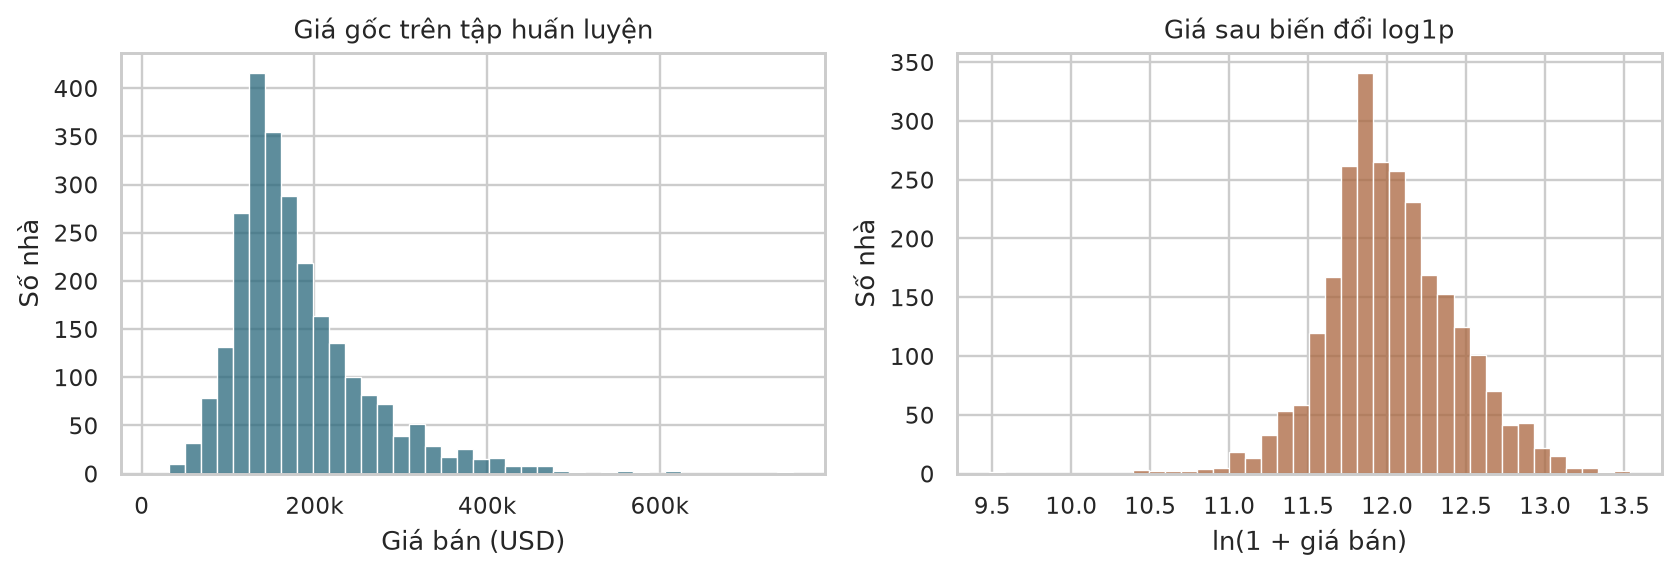
\includegraphics[width=1\linewidth]{01_target.png}
\caption{Phân bố giá trước và sau log1p}\end{figure}

Độ lệch mẫu của giá là 1.738; sau log1p còn 0.055. Biến đổi giảm đáng kể đuôi phải và chênh lệch thang giá. Tuy nhiên, phân bố mục tiêu gần đối xứng không bảo đảm phần dư mô hình có phương sai không đổi hoặc phân bố chuẩn. Cần kiểm tra phần dư khi có mô hình ở KT2.


\begin{figure}[H]\centering
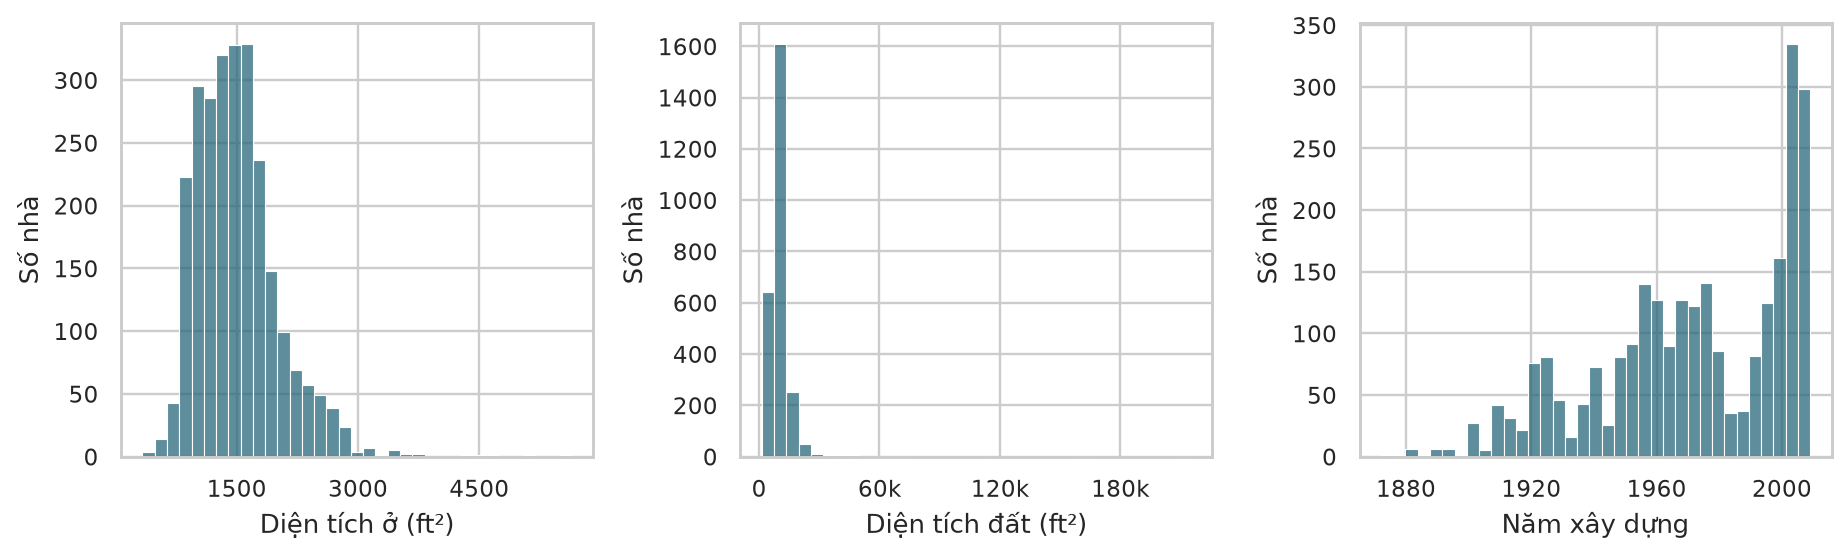
\includegraphics[width=1\linewidth]{02_features.png}
\caption{Phân bố các đặc trưng chính trên train}\end{figure}

Diện tích ở có đuôi phải; diện tích đất có một số lô rất lớn làm trục kéo dài. Điều này tạo rủi ro điểm có đòn bẩy lớn đối với hồi quy tuyến tính. Năm xây dựng trải qua nhiều thời kỳ, gợi ý giá chịu ảnh hưởng đồng thời của độ mới và chất lượng nhà. Không quy mọi nhà lớn hoặc nhà cũ thành dữ liệu sai.


\clearpage

\section{Quan hệ giữa đặc trưng và giá}

\begin{figure}[H]\centering
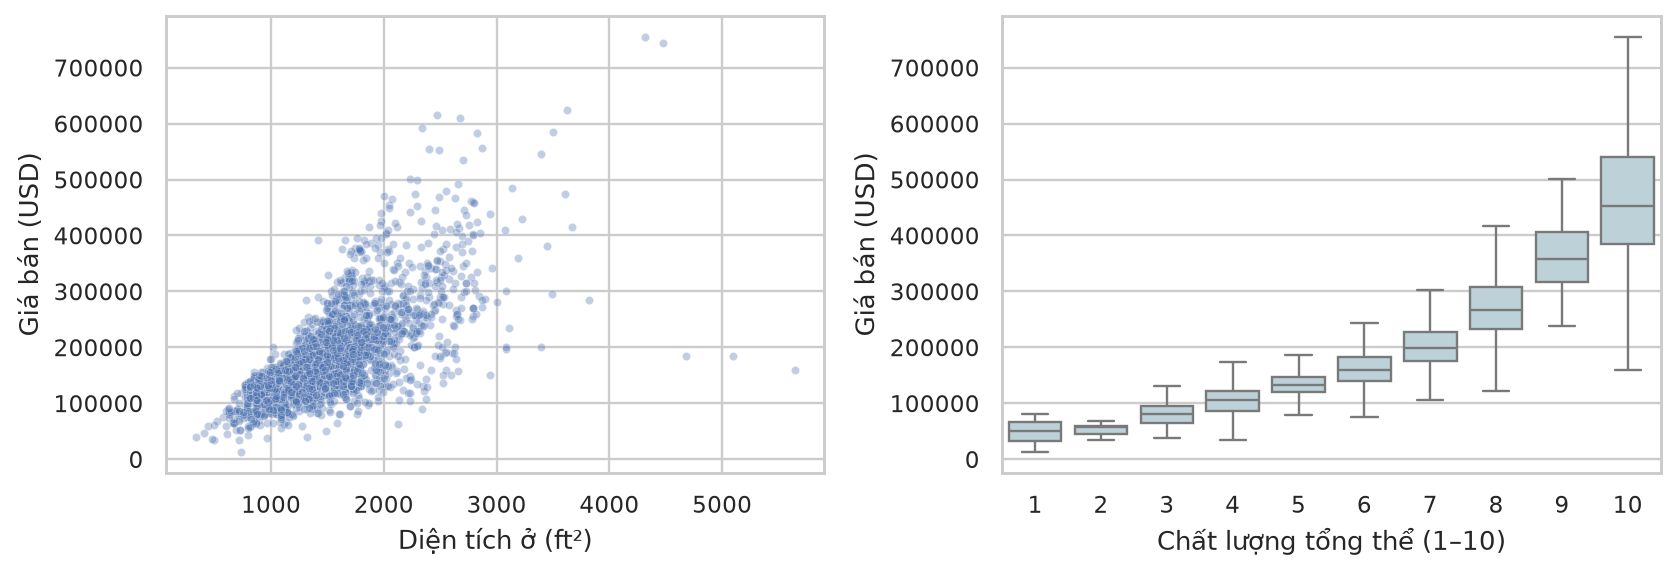
\includegraphics[width=1\linewidth]{03_relationships.png}
\caption{Diện tích ở và chất lượng tổng thể so với giá}\end{figure}

Diện tích ở có tương quan Pearson 0.709 với giá trên train. Xu hướng tăng rõ nhưng cùng diện tích vẫn có nhiều mức giá. Giữ diện tích ở làm đầu vào, đồng thời bổ sung chất lượng và khu vực thay vì xây mô hình chỉ theo diện tích. Có 5 nhà trên 4.000 ft\textsuperscript{2} trong train; cần xem từng mẫu, không tự động xóa theo một ngưỡng diện tích.


Overall Qual có tương quan 0.802 với giá. Các hộp phân bố dịch lên khi mức chất lượng tăng, hỗ trợ giữ biến này. Cấu hình đầu tiên xem điểm 1–10 là số để giữ thứ tự, đồng thời thừa nhận giả định khoảng cách điểm tương đương có thể chưa phản ánh đầy đủ quan hệ giá.


\begin{figure}[H]\centering
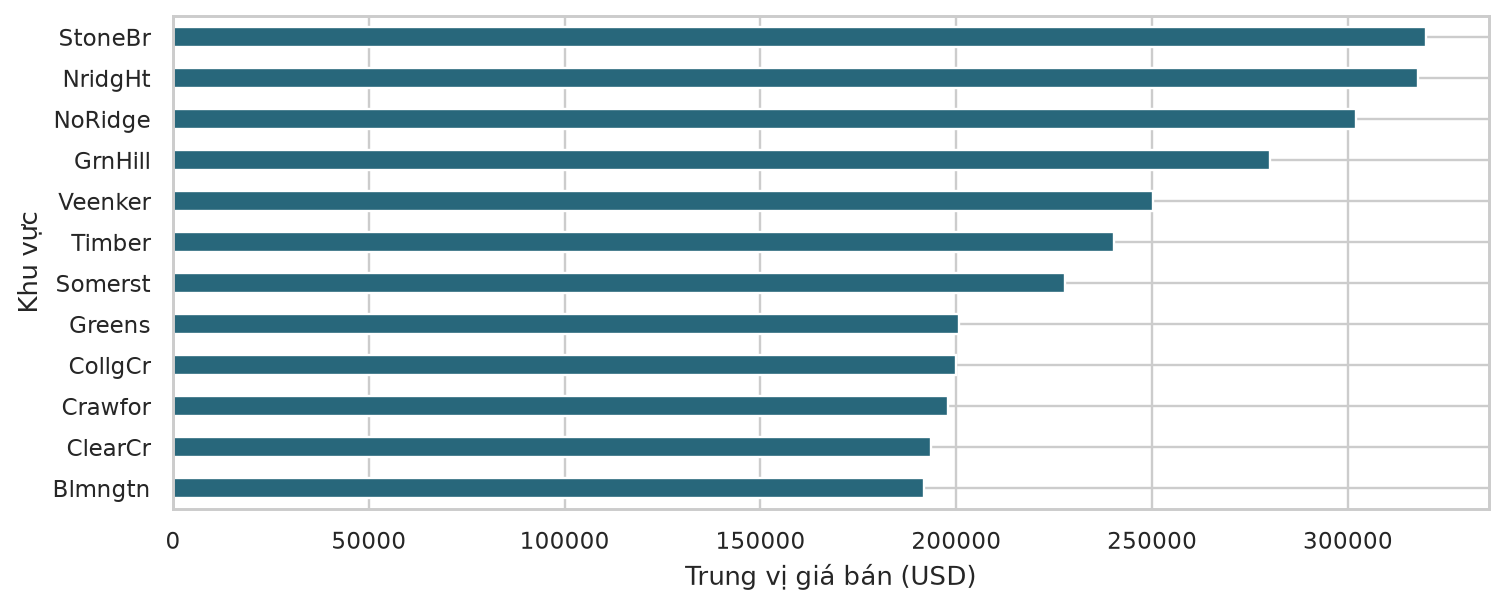
\includegraphics[width=1\linewidth]{07_neighborhood.png}
\caption{Trung vị giá theo 12 khu vực có trung vị cao nhất trên train}\end{figure}

Trung vị giá khác nhau giữa các khu vực. Vì vậy, Neighborhood cần được mã hóa và giữ lại trong mô hình. Mức trung vị ở nhóm nhỏ có độ bất định cao; notebook đi kèm cả số mẫu theo khu vực. Không dùng biểu đồ này như bằng chứng nhân quả hoặc khẳng định một khu vực luôn đắt hơn khi mọi đặc điểm khác giữ nguyên.


\clearpage

\section{Tương quan và động cơ chính quy hóa}

\begin{figure}[H]\centering
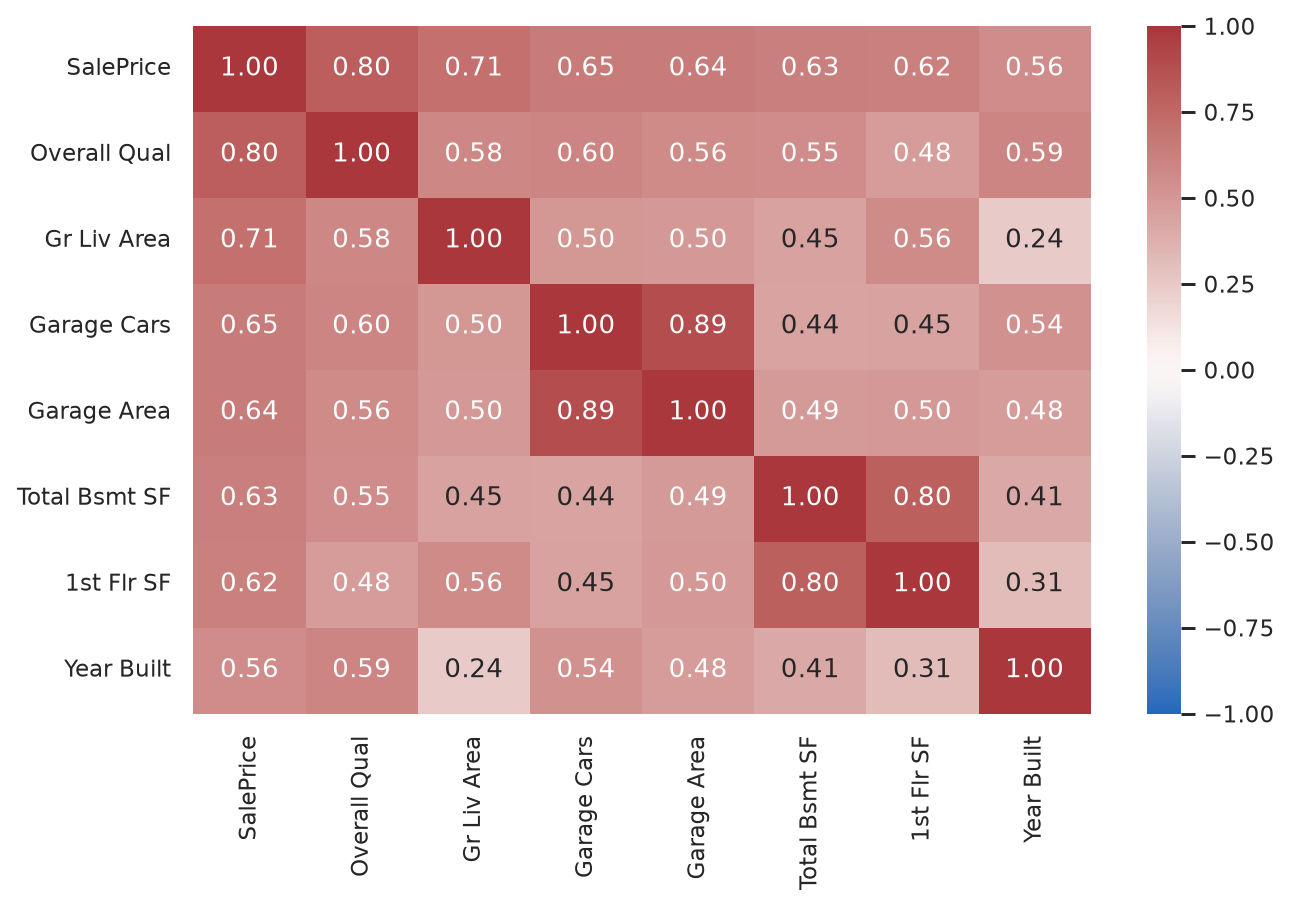
\includegraphics[width=.93\linewidth]{04_correlations.png}
\caption{Ma trận tương quan Pearson trên train}\end{figure}

Garage Cars tương quan 0.648 với giá; năm xây dựng tương quan 0.556. Hai biến đều cung cấp tín hiệu hợp lý nhưng không nên được diễn giải là tác động riêng biệt khi chưa điều chỉnh các yếu tố khác.


Garage Area và Garage Cars có tương quan 0.888. Hai phép đo cùng phản ánh quy mô garage, tạo đa cộng tuyến. Hệ số OLS có thể nhạy với nhiễu hoặc thay đổi mẫu dù dự đoán tổng thể vẫn tương đối ổn định. Ridge có thể làm hệ số ổn định hơn; Lasso có thể chọn một trong các biến tương quan; Elastic Net kết hợp co hệ số và độ thưa. Hiệu quả thực tế vẫn phải được kiểm chứng bằng CV.


Ba kết luận để xây dựng mô hình là giữ thông tin chất lượng; sử dụng diện tích cùng các yếu tố vị trí và tiện ích; và so sánh chính quy hóa khi có các biến liên quan mạnh. Chưa loại biến chỉ dựa trên tương quan với nhãn, vì một biến có tương quan biên thấp vẫn có thể bổ sung thông tin khi kết hợp với biến khác.


Pearson phản ánh chủ yếu quan hệ tuyến tính và nhạy với ngoại lai. Ma trận này dùng các biến số, không đánh giá đầy đủ các cột phân loại. Quan hệ giữa khu vực và giá được khảo sát bổ sung bằng thống kê nhóm. Không tính tương quan từ tập test để chọn mô hình.


\clearpage

\section{Phát hiện vấn đề chất lượng dữ liệu}

Audit cấu trúc trên toàn bộ raw dùng để xác định schema và ghi nhận chất lượng; quyết định và thống kê học được của pipeline chỉ dùng train. Mỗi cột có số mã NA, ô trống, kiểu và số giá trị duy nhất trong \path{quality_all_columns.csv}.


\begingroup\small\setlength{\tabcolsep}{5pt}
\begin{tabularx}{\linewidth}{@{}YYY@{}}\toprule

\textbf{Vấn đề} & \textbf{Định lượng thực tế} & \textbf{Ý nghĩa}\\

\midrule

Ô trống thực sự & 719 ô & Thiếu thông tin, cần xử lý\\

Literal NA & 13,278 ô ở 14 cột & Nghĩa không có tiện ích theo từ điển\\

Trùng nguyên dòng & 0 & Không cần xóa\\

Trùng sau bỏ Order và PID & 0 & Không phát hiện giao dịch lặp nội dung\\

PID lặp & 0 & Không có cùng thửa đất ở hai tập\\

Ô chuỗi có khoảng trắng thừa & 2,536 & Cần strip, gồm mã giao dịch bị loại\\

Năm vượt năm bán hoặc trước 1800 & 6 ô & 1 Year Built, 3 Year Remod/Add, 2 Garage Yr Blt\\

Nhà trên 4.000 ft\textsuperscript{2} & 5 mẫu train & Cờ kiểm tra, không tự coi là sai\\

\bottomrule\end{tabularx}\endgroup\par

\begin{figure}[H]\centering
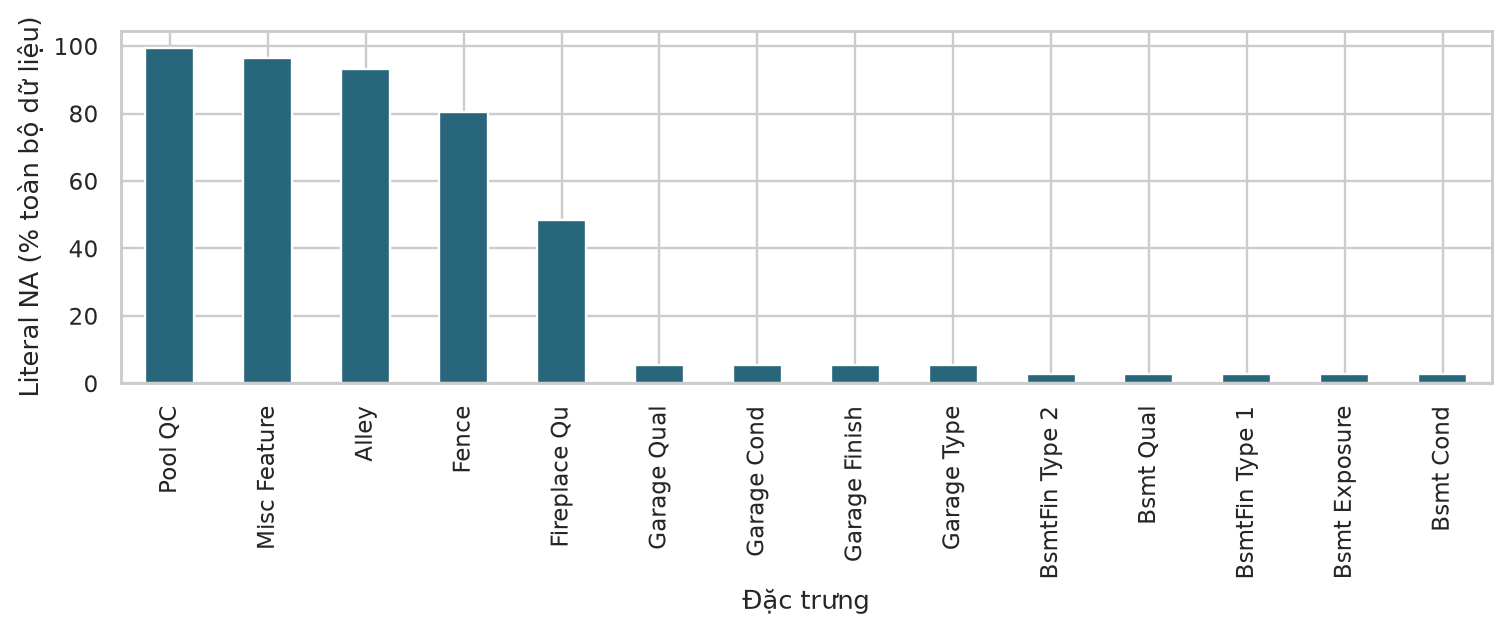
\includegraphics[width=1\linewidth]{05_na_tokens.png}
\caption{Tỷ lệ literal NA ở các cột trên toàn bộ raw}\end{figure}

Pool QC, Misc Feature và Alley có nhiều mã NA vì đa số nhà không có các tiện ích đó. Xóa các cột chỉ vì tỷ lệ NA cao sẽ đánh mất thông tin hiện diện/không hiện diện. Các ô trống trong cùng cột vẫn là thiếu thật. None ở Mas Vnr Type là mã hợp lệ và được giữ nguyên.


Bảng \path{outliers_iqr_train.csv} định lượng cờ ngoại lai theo Q1\ensuremath{-}1,5\ensuremath{\times}IQR và Q3+1,5\ensuremath{\times}IQR cho từng biến số. Với biến rời rạc hoặc nhiều số 0, IQR có thể nhỏ hoặc bằng 0; cờ chỉ dùng rà soát, không phải lệnh xóa. Bài toán hồi quy không có mất cân bằng lớp; thay vào đó cần chú ý ít mẫu ở đuôi giá cao. Rủi ro rò rỉ gồm nhãn/ID, thông tin chốt giao dịch và preprocessing học từ validation/test.


\clearpage

\section{Xử lý dữ liệu và đối chiếu trước sau}

Các quy tắc cố định gồm strip chuỗi; giữ mã None; chuyển NA chỉ không có tiện ích thành \_\_ABSENT\_\_; chuyển ô trống thành thiếu. MS SubClass được đọc dạng chuỗi để không mất mã loại nhà. Tháng bán được xem là phân loại. Sáu ô năm vi phạm giả định thời điểm được chuyển sang thiếu; đây là quy tắc làm sạch có chủ ý, không phải khẳng định mọi trường hợp đều là lỗi nhập liệu.


Đối với biến số, điền median học trên train và thêm chỉ báo thiếu. Chỉ báo giúp phân biệt giá trị quan sát với giá trị điền. Việc điền năm garage khi nhà không có garage chỉ là biểu diễn kỹ thuật; sự vắng mặt được thể hiện thêm qua các biến phân loại. Với biến phân loại, ô thiếu thật thành \_\_MISSING\_\_, tách biệt \_\_ABSENT\_\_.


Các cột diện tích và Misc Val được clip trong khoảng từ 0 đến phân vị 99\% học trên train. Không clip năm, điểm chất lượng, số xe, số phòng hoặc nhãn giá. Danh sách cột và số ô thay đổi từng tập nằm ở \path{clipping_audit.csv}. Không xóa dòng, vì ngoại lai có thể là giao dịch hợp lệ.


\begin{figure}[H]\centering
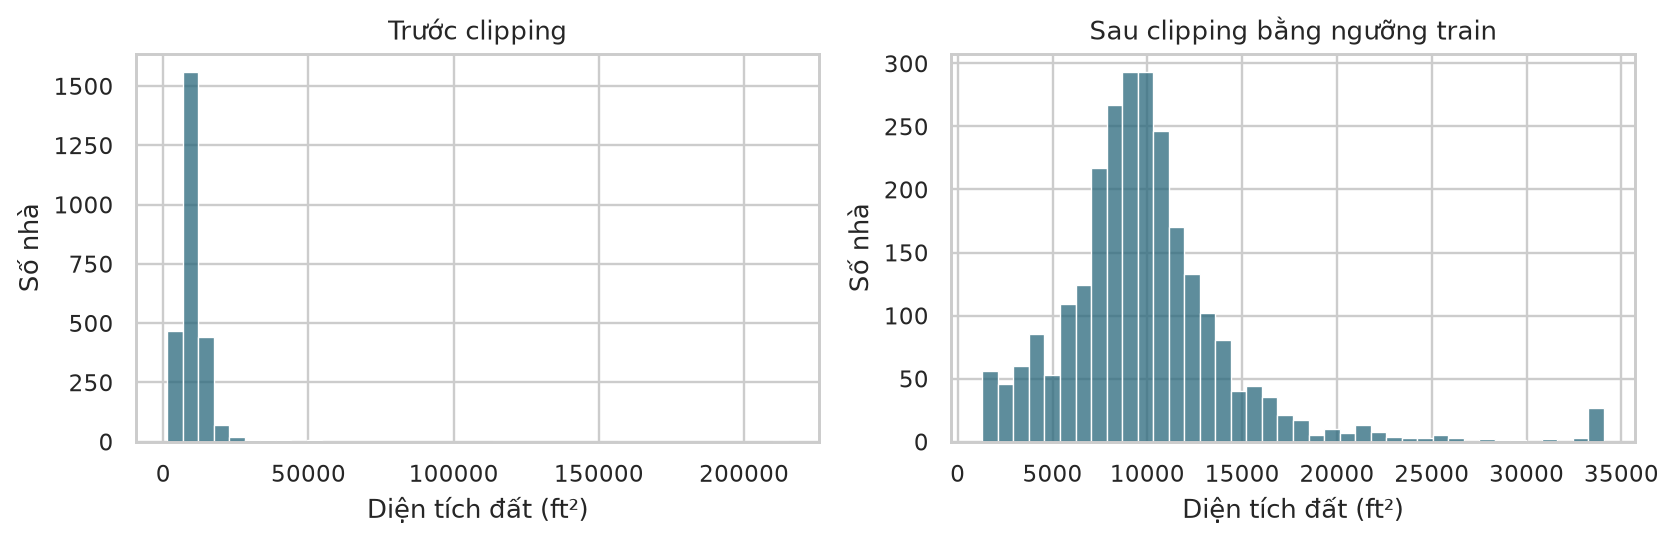
\includegraphics[width=1\linewidth]{06_before_after.png}
\caption{Phân bố diện tích đất trước và sau clipping trên train}\end{figure}

Clipping giảm độ dài đuôi và ảnh hưởng của lô cực lớn nhưng làm mất một phần khác biệt ở đuôi trên. Cấu hình này chưa được chứng minh tối ưu; KT2/3 phải so sánh có/không clipping trên cùng CV, không chỉnh ngưỡng theo kết quả test.


\begingroup\small\setlength{\tabcolsep}{5pt}
\begin{tabularx}{\linewidth}{@{}Yrrr@{}}\toprule

\textbf{Giai đoạn} & \textbf{Dòng} & \textbf{Cột} & \textbf{Số ô thiếu}\\

\midrule

Train sau quy tắc ngữ nghĩa & 2.589 & 77 & 648\\

Test sau quy tắc ngữ nghĩa & 341 & 77 & 77\\

Train sau pipeline & 2.589 & 350 & 0\\

Test sau pipeline & 341 & 350 & 0\\

\bottomrule\end{tabularx}\endgroup\par

Tổng số ô thiếu sau quy tắc là 725, bằng 719 ô trống cộng 6 ô năm bị chuyển thành thiếu. Số cột tăng do one-hot và cờ thiếu. Tính hữu hạn của hai ma trận được kiểm tra tự động.


\clearpage

\section{Chuẩn bị dữ liệu và chiến lược đánh giá}

\subsection{Pipeline và chống rò rỉ}

Chia dữ liệu theo năm trước EDA và trước fit preprocessing. Năm 2006 có 625 mẫu, 2007 có 694 mẫu, 2008 có 622 mẫu, 2009 có 648 mẫu và 2010 có 341 mẫu. Train là 2006–2009, test là 2010; đây là phép chia tất định nên không phụ thuộc seed. SEED=42 được giữ cho các bước ngẫu nhiên ở mốc sau.


Pipeline gồm QuantileClipper và ColumnTransformer. Nhánh số có SimpleImputer với median và cờ thiếu rồi StandardScaler. Nhánh phân loại có điền hằng số và OneHotEncoder với quy tắc ignore cho mức mới. Chuẩn hóa số giúp mức phạt hệ số ít phụ thuộc đơn vị. One-hot giữ 0/1; giữ đủ mức để diễn giải với regularization, chấp nhận các quan hệ phụ thuộc tuyến tính mà OLS cần xử lý bằng nghiệm bình phương tối thiểu phù hợp.


Lệnh fit\_transform chỉ áp dụng train, transform áp dụng test. Không đưa SalePrice vào bộ biến đổi X. log1p là hàm cố định của nhãn, không học thống kê. Nếu mô hình tạo dự đoán âm sau hoàn nguyên, quy tắc đánh giá dự kiến là chặn giá tại 0 và báo cáo rõ quy tắc này. Tối ưu trên log không bảo đảm trung bình dự đoán USD không chệch.


\subsection{Kiểm định chéo cho mốc tiếp theo}

\begingroup\small\setlength{\tabcolsep}{5pt}
\begin{tabularx}{\linewidth}{@{}cYYrr@{}}\toprule

\textbf{Fold} & \textbf{Năm học} & \textbf{Năm kiểm định} & \textbf{Số mẫu học} & \textbf{Số mẫu kiểm định}\\

\midrule

1 & 2006 & 2007 & 625 & 694\\

2 & 2006–2007 & 2008 & 1.319 & 622\\

3 & 2006–2008 & 2009 & 1.941 & 648\\

\bottomrule\end{tabularx}\endgroup\par

Ba fold mở rộng mô phỏng học quá khứ để dự báo tương lai, phù hợp hơn chia ngẫu nhiên với định hướng sử dụng của dự án. Trong mỗi fold phải khởi tạo và fit lại cả preprocessing từ dữ liệu gốc. Tính trung bình, độ lệch chuẩn và kết quả từng fold; ghi rõ nếu lấy trung bình không trọng số giữa các năm. Chỉ ba fold và năm 2010 chưa đủ toàn năm là hạn chế của đánh giá.


Không dùng ma trận \path{ames_ready.npz} đã fit toàn train để tính CV. Với RidgeCV/LassoCV, đặt sau preprocessing đã fit cả train vẫn có thể rò rỉ giữa các fold nội bộ. KT2 cần vòng ngoài fit lại toàn pipeline cho mỗi cấu hình alpha và mỗi fold theo năm; việc dùng các lớp CV phải được giải thích rõ giới hạn này. Chọn cấu hình xong mới fit lại trên 2006–2009 và đánh giá cuối trên 2010 một lần.


\clearpage

\section{Cơ sở toán học của chính quy hóa}

Phần này chuẩn bị lý thuyết cho đề tài; KT1 chưa tối ưu hệ số hay chọn
$\alpha$. Gọi $X\in\R^{n\times p}$ là ma trận đặc trưng sau biến đổi,
$w\in\R^p$ là hệ số, $b$ là intercept và $z=\ln(1+y)$.
Intercept thường không bị phạt. Sử dụng quy ước mất mát chuẩn hóa theo $1/(2n)$.


\begin{equation}
J(w,b)=\frac{1}{2n}\lVert z-b\bm 1-Xw\rVert_2^2
+\alpha\left[\rho\lVert w\rVert_1+\frac{1-\rho}{2}\lVert w\rVert_2^2\right].
\label{eq:elastic}
\end{equation}
\begin{equation}
\widehat{w}_{\mathrm{L2}}=
\left(\frac{X^{\mathsf T}X}{n}+\alpha I\right)^{-1}
\frac{X^{\mathsf T}z}{n}.
\label{eq:ridge}
\end{equation}


Với L2, đặt gradient theo $w$ bằng 0 sau khi tâm hóa $X$ và $z$ thu được
\[
\left(\frac{X^{\mathsf T}X}{n}+\alpha I\right)w=\frac{X^{\mathsf T}z}{n}.
\]
Khi $\alpha>0$, phần $\alpha I$ làm các hướng có trị riêng nhỏ ổn định hơn.
Hệ số thường co liên tục và không thành đúng 0. Điều này phù hợp khi nhiều
biến có tín hiệu nhỏ hoặc các biến garage và diện tích liên quan mạnh.

Với L1, chuẩn trị tuyệt đối không khả vi tại 0. Điều kiện tối ưu dùng
dưới gradient, cho phép một số hệ số bằng đúng 0. Trong trường hợp đặc biệt
$X^{\mathsf T}X/n=I$, nghiệm là soft-threshold:
\begin{equation}
w_j=\operatorname{sign}(c_j)\max(|c_j|-\alpha,0),\qquad
c=\frac{X^{\mathsf T}z}{n}.
\end{equation}
Công thức giải thích cơ chế chọn biến nhưng không phải nghiệm đóng cho
dữ liệu Ames tổng quát.

Elastic Net kết hợp L1 và L2 qua \ensuremath{\rho}, tương ứng l1\_ratio. Khi \ensuremath{\rho} = 1 là Lasso; khi \ensuremath{\rho} = 0 là L2 theo quy ước trên. Với 0 < \ensuremath{\rho} < 1, mô hình vừa có khả năng tạo độ thưa vừa ổn định hơn khi các đặc trưng tương quan. Trong triển khai, trường hợp L2 thuần nên dùng Ridge thay vì ép ElasticNet với l1\_ratio=0.


Alpha kiểm soát tổng mức phạt. Alpha nhỏ gần OLS; alpha lớn thường giảm độ lớn hệ số, giảm phương sai nhưng tăng độ chệch. Giá trị quá lớn có thể gây thiếu khớp. Không có alpha tốt nhất độc lập với dữ liệu, cách scale và chỉ số. Ở scikit-learn, Ridge dùng SSE + alpha\_ridge||w||\textsuperscript{2}, nên cùng quy ước L2 trên thì alpha\_ridge = n\ensuremath{\alpha}. Không so sánh trực tiếp cùng số alpha giữa Ridge và Lasso/Elastic Net [4].


Giai đoạn sau sẽ so sánh OLS, Ridge, Lasso và Elastic Net; tìm alpha trên lưới log riêng từng thuật toán, và thêm l1\_ratio cho Elastic Net. Chưa khẳng định mô hình nào tốt nhất trước khi có kết quả kiểm định.


\clearpage

\section{Minh chứng hoàn thành và thực hành cá nhân}

\subsection{Đối chiếu yêu cầu KT1}

\begingroup\small\setlength{\tabcolsep}{5pt}
\begin{tabularx}{\linewidth}{@{}YY@{}}\toprule

\textbf{Tiêu chí} & \textbf{Vị trí minh chứng chính}\\

\midrule

1 Phát biểu bài toán & Mục 1 và notebook mục 1\\

2 Mục tiêu và chỉ số & Bảng mục tiêu ở mục 1\\

3 Nguồn và từ điển & Mục 2, \path{SOURCES.md}, \path{data_dictionary.csv}\\

4 Thống kê và phân bố & Mục 3, hình 1–2, bảng mô tả đầy đủ\\

5 Quan hệ và nhận xét & Mục 4–5, hình 3–5\\

6 Định lượng vấn đề & Mục 6, \path{quality_all_columns.csv}, \path{outliers_iqr_train.csv}\\

7 Xử lý và trước sau & Mục 7, \path{preprocessing.py}, \path{clipping_audit.csv}\\

8 Chuẩn bị dữ liệu đúng & Mục 8, notebook, \path{split_manifest.csv}\\

9 Lý giải đánh giá cá nhân & Mục 8 và thực hành vấn đáp\\

10 Thực hành cá nhân & \path{ON_TAP_VAN_DAP.md} và thao tác trực tiếp\\

\bottomrule\end{tabularx}\endgroup\par

Notebook đã được chạy từ đầu đến cuối và lưu đầu ra. Ba kiểm tra tự động xác nhận schema/giữ nghĩa NA, độ ổn định khi transform mã mới và dữ liệu cực trị, cùng tính đúng của log1p/expm1. Các kiểm tra này hỗ trợ tính đúng quy trình, không thay thế đánh giá mô hình.


\subsection{Gợi ý thực hành tại chỗ}

Sinh viên cần tự thống kê lại Lot Frontage; vẽ quan hệ Gr Liv Area–SalePrice; đổi median sang mean và fit lại chỉ trên train; đổi ngưỡng clipping để quan sát số ô thay đổi. Cần giải thích vì sao NA tiện ích khác ô trống, vì sao không dùng năm 2010 để chọn alpha và vì sao ma trận đã fit toàn train không dùng trực tiếp cho CV.


Tài liệu \path{ON_TAP_VAN_DAP.md} có câu hỏi, gợi ý trả lời và các đoạn mã dùng trực tiếp với biến trong notebook. Kết quả tiêu chí cá nhân phụ thuộc khả năng giải thích và thao tác của sinh viên, không được suy ra chỉ từ việc có tài liệu.


\subsection{Khai báo công cụ và đóng góp}

Codex AI được sử dụng để tìm nguồn, soạn mã tải/khảo sát/tiền xử lý, chạy kiểm tra và chuẩn bị notebook cùng báo cáo. Sinh viên có trách nhiệm kiểm tra tính đúng, trích dẫn và hiểu nội dung trước khi nộp. Họ tên, MSSV, lớp và phân công thực tế cần được bổ sung. Không tự tạo đóng góp cá nhân hoặc lịch sử công việc chưa xảy ra. Nhật ký hiện có ghi rõ phần chuẩn bị bằng AI; sinh viên bổ sung các lần tự kiểm tra và sửa thực tế.


\clearpage

\section{Hạn chế và kế hoạch tiếp theo}

Dữ liệu thuộc một thành phố và giai đoạn lịch sử, vì vậy kết quả sau này chỉ có ý nghĩa trong bối cảnh đánh giá đã xác định. Test năm 2010 có 341 giao dịch và chưa đại diện đầy đủ mọi mùa trong năm. Không thể dùng bài này để định giá bất động sản Việt Nam hoặc quy đổi thành giá hiện tại chỉ bằng tỷ giá.


Chất lượng tổng thể và các đánh giá vật liệu có thể chủ quan; thời điểm thu thập cần được xác minh khi đưa vào ứng dụng thực tế. Một số tổ hợp biến có thông tin trùng nhau. Clipping có thể làm giảm khả năng dự đoán nhà hiếm ở đuôi giá cao. Cờ thiếu giúp mô hình nhận biết giá trị điền nhưng không khôi phục thông tin chưa được ghi nhận. Việc one-hot mức chưa gặp thành toàn 0 là phương án kỹ thuật có giới hạn, cần theo dõi drift.


Ở KT2, bổ sung baseline, huấn luyện bốn mô hình theo cùng các fold thời gian, chọn alpha trên train, báo cáo RMSE log, MAE/RMSE USD, R\textsuperscript{2} và phân tích phần dư. So sánh sai số theo nhóm diện tích, chất lượng và mức giá. Ở KT3, đánh giá tác động có/không clipping, các đặc trưng tuổi nhà hoặc tổng diện tích và cách mã hóa thứ bậc. Tập test giữ nguyên để tránh chọn phương án theo kết quả cuối.


\subsection*{Tài liệu tham khảo}

[1] De Cock, D. (2011). Ames, Iowa: Alternative to the Boston Housing Data as an End of Semester Regression Project. Journal of Statistics Education, 19(3). DOI: \url{https://doi.org/10.1080/10691898.2011.11889627}. Bản trên JSE: \url{https://jse.amstat.org/v19n3/decock.pdf}


[2] De Cock, D. \path{AmesHousing.txt}. \url{https://jse.amstat.org/v19n3/decock/AmesHousing.txt}. Truy cập ngày 26/10/2026.


[3] De Cock, D. \path{DataDocumentation.txt}. \url{https://jse.amstat.org/v19n3/decock/DataDocumentation.txt}. Truy cập ngày 26/10/2026.


[4] Scikit-learn developers. Linear Models và Common pitfalls. \url{https://scikit-learn.org/stable/modules/linear_model.html} và \url{https://scikit-learn.org/stable/common_pitfalls.html}. Truy cập ngày 26/10/2026. Môi trường chạy đã khóa phiên bản trong \path{requirements.txt}.


[5] Bộ tiêu chí đánh giá dự án học máy, học kỳ 1 năm học 2026–2027, bản người học cung cấp. Dùng để xác định phạm vi và minh chứng KT1; không dùng làm nguồn dữ liệu thực nghiệm.


\end{document}